\section{Previous Searches for Higgs Boson Pair Production}%
\label{seq:experimental_status}

The following summarises the experimental status of searches for Higgs boson
pair production prior to the work performed as part of this thesis. The focus
lies on results of the ATLAS and CMS collaborations obtained using \pp~collision
datasets at $\sqrt{s} = \SI{13}{\TeV}$ collected during the 2015 and 2016
data-taking periods at the LHC.


\subsection*{Searches for SM Higgs Boson Pair Production}%
\label{sec:past_results_smhh}

% https://cms-results.web.cern.ch/cms-results/public-results/publications/HIG-17-030/index.html

The ATLAS and CMS collaborations set upper limits on the cross section of SM \HH
production via \ggF, $\sigma_{\ggF}$, at \SI{95}{\percent} CL. The results of
both collaborations are summarised in \Cref{fig:prior_status_smhh}. Searches for
SM \HH production were performed in various channels, the \bbbb, \bbtautau, and
\bbyy channels being the most sensitive ones. A statistical combination of SM
\HH searches was performed by both collaborations. The observed (expected) upper
limits on $\sigma_{\ggF} / \sigma_{\ggF}^{\text{SM}}$ of the combination are
$6.9$ ($10$) and $22.2$ ($12.8$) ATLAS and CMS collaboration,
respectively~\cite{HDBS-2018-58,CMS-HIG-17-030}. These were the most stringent
limits on SM~\HH production at the time.

\begin{figure}[htbp]
  \centering

  \begin{subfigure}[b]{0.9\textwidth}
    \centering

    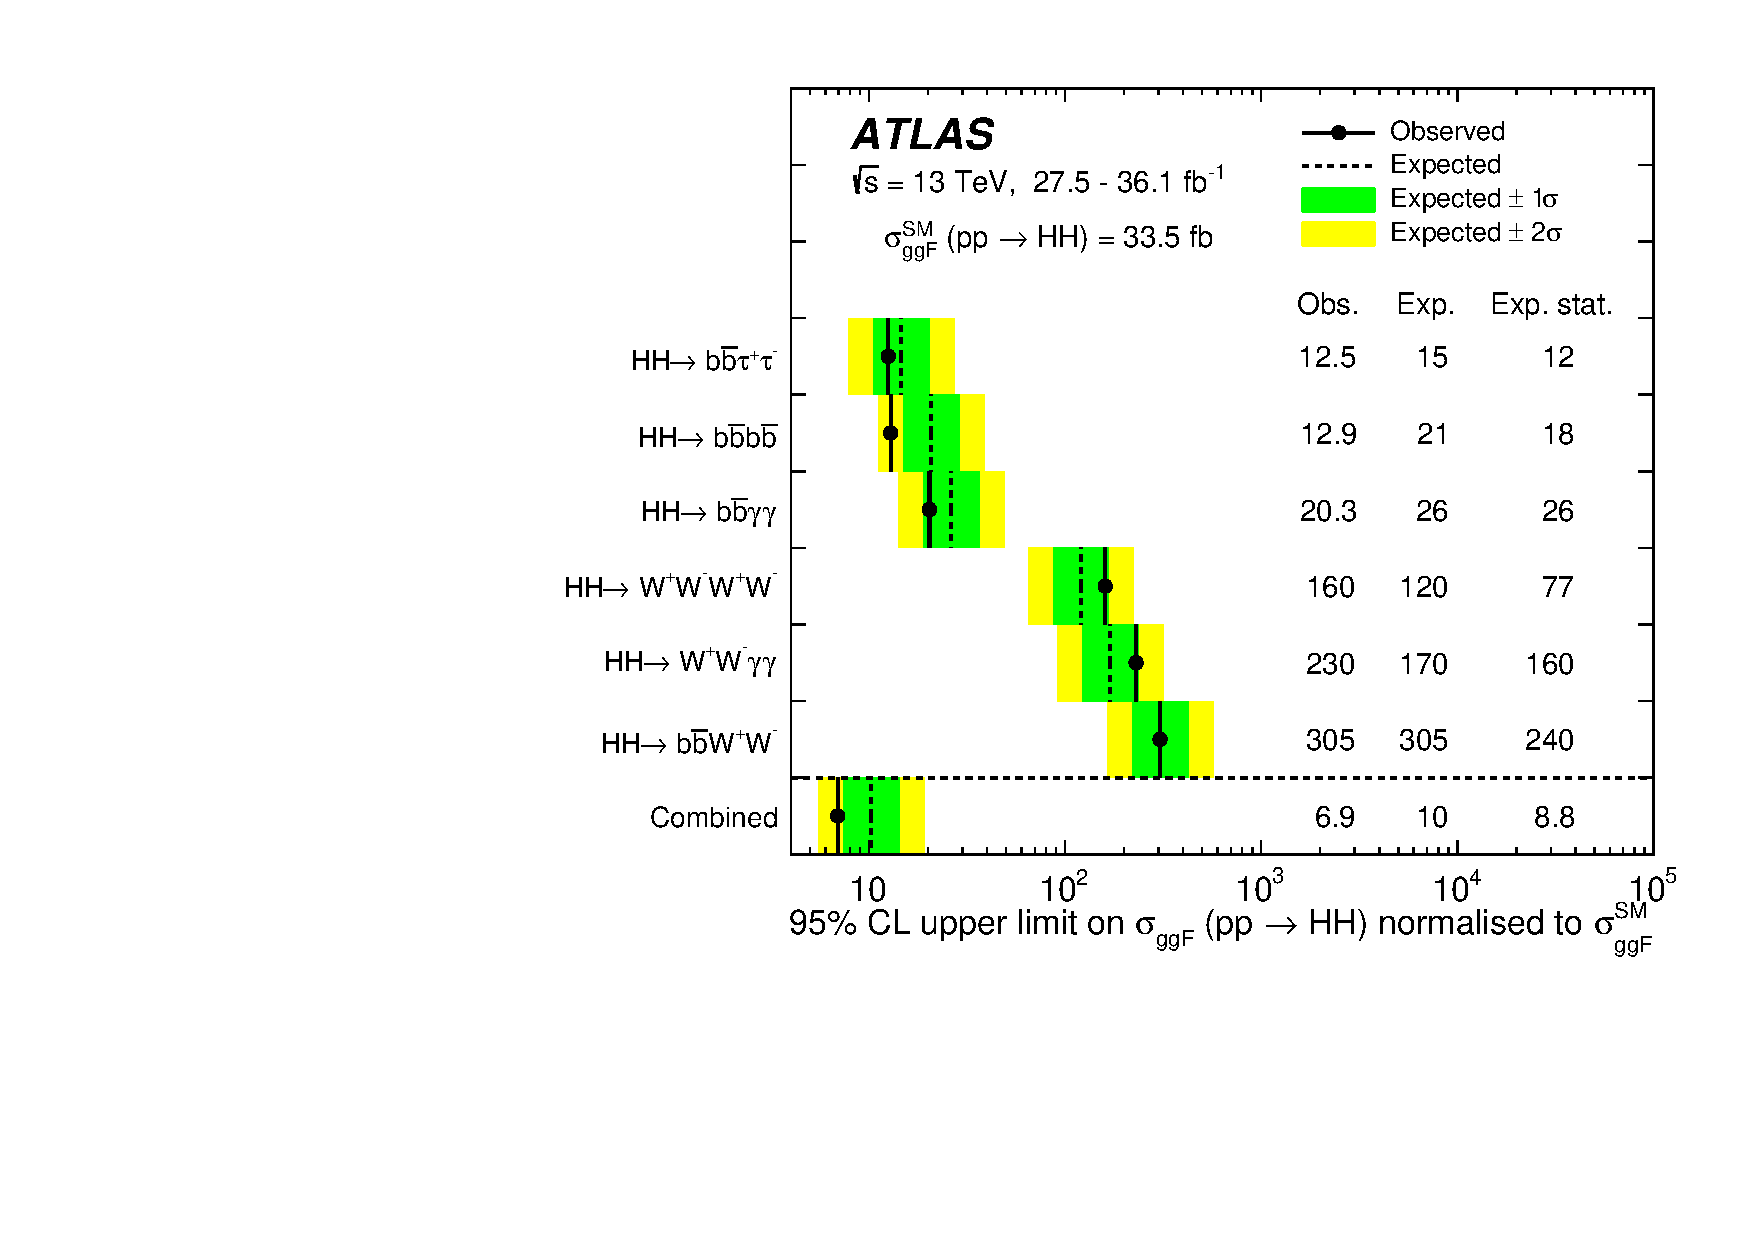
\includegraphics[width=0.62\textwidth, trim=0 0.4em 0 0,
    clip]{status/atlas_36ifb}

    \subcaption{Results of SM \HH searches by the ATLAS collaboration.  Upper
      limits excluding systematic uncertainties are given in the ``Exp.\ stat.''
      column.  The figure is taken from Ref.~\cite{HDBS-2018-58}.}
  \end{subfigure}

  \vspace{0.5em}

  \begin{subfigure}[b]{0.9\textwidth}
    \centering

    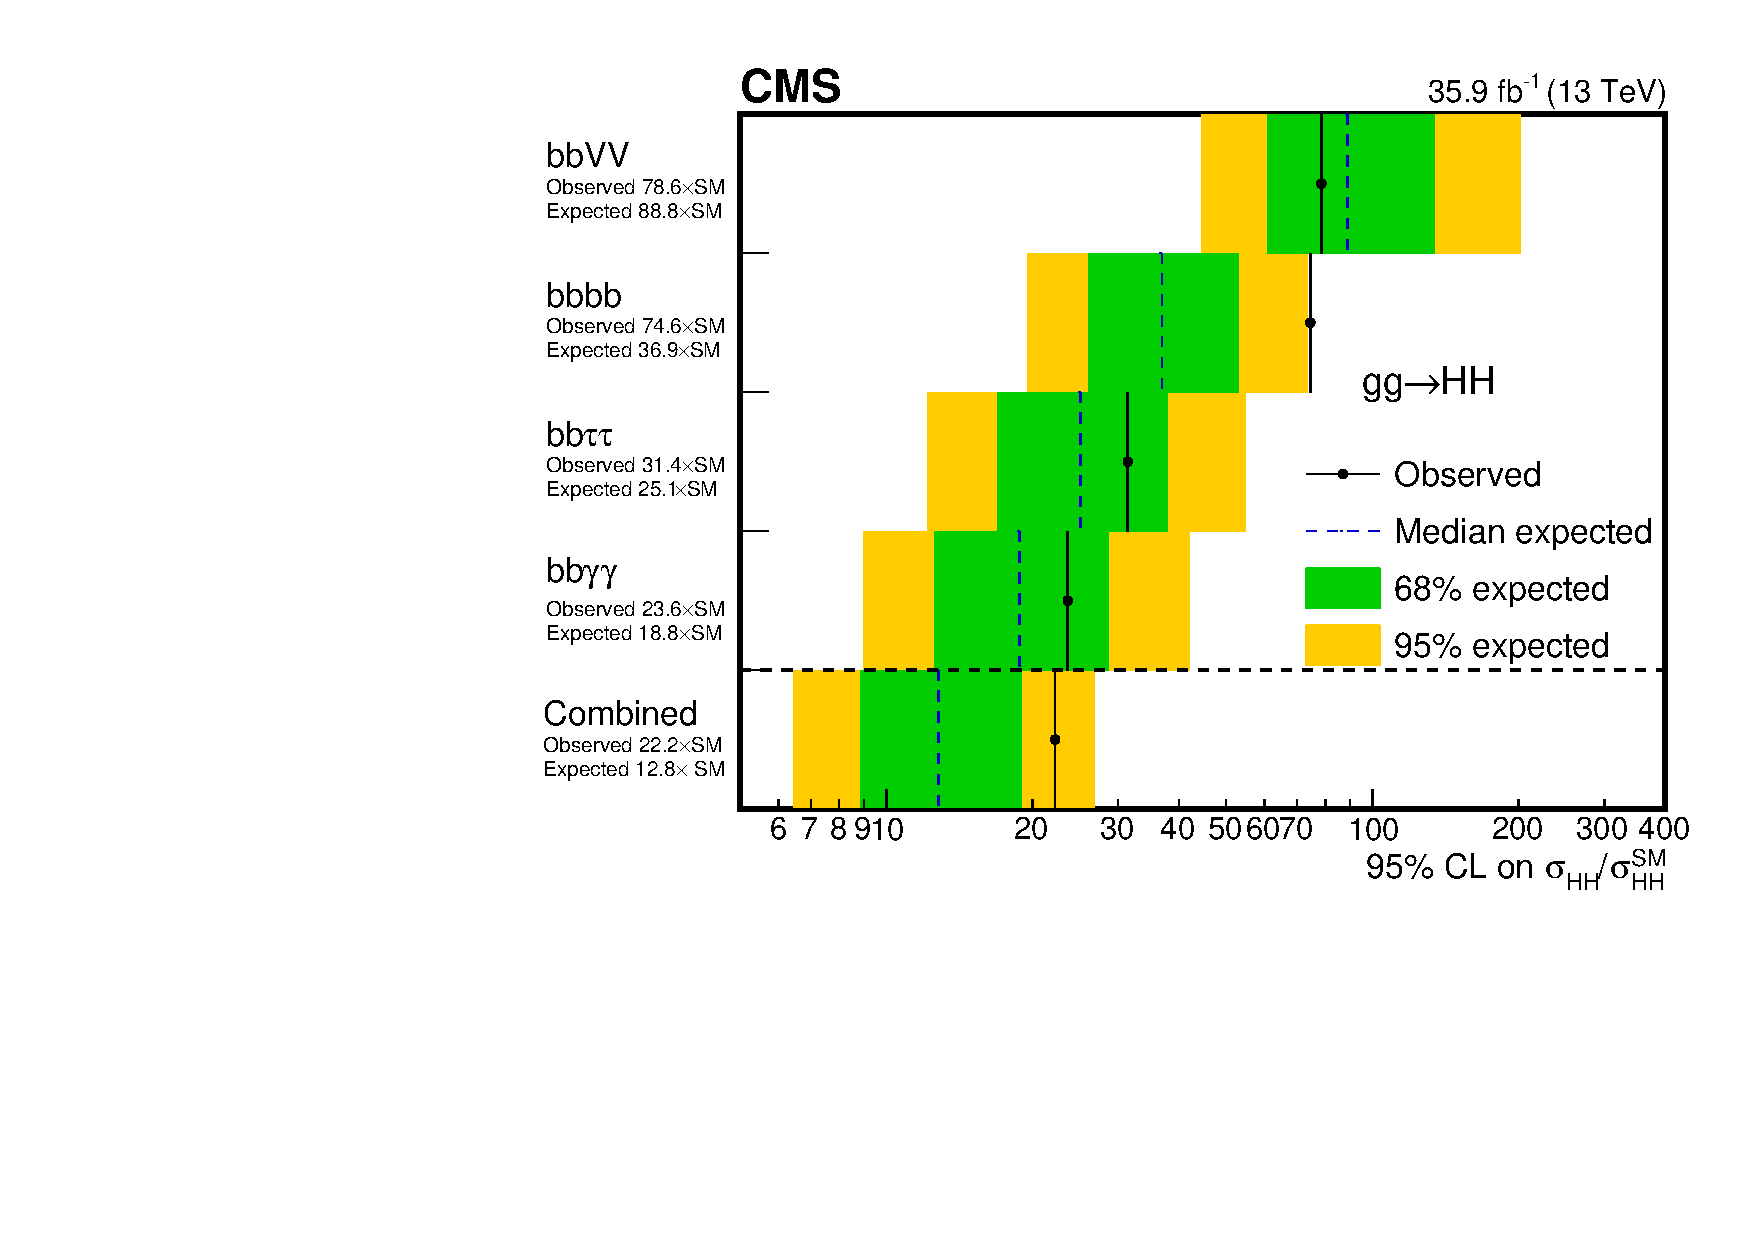
\includegraphics[width=0.62\textwidth]{status/cms_36ifb}

    \subcaption{Results of SM \HH searches by the CMS collaboration. The
      $\bbbar V V$ ($V = Z$ or $W^\pm$) channel targets final states with two
      charged leptons. The figure is taken from Ref.~\cite{CMS-HIG-17-030}.}
  \end{subfigure}

  \caption[Upper limits on the SM~\HH production cross section by the ATLAS and
  CMS collaborations based on \pp~collision data taken in 2015 and 2016.]{Upper
    limits at \SI{95}{\percent} CL on the cross section of SM \HH production via
    \ggF by the ATLAS (a) and CMS (b) collaborations. The upper limits are
    normalised to a SM cross section prediction of
    $\sigma_{\ggF} = \SI{33.5}{\femto\barn}$ and given separately for the
    individual channels, and the statistical combination of all listed
    channels. In both cases, the expected limits are derived under the
    background-only hypothesis (i.e.\ no SM \HH production). The results are
    based on \pp~collision data taken in 2015 and 2016.}%
  \label{fig:prior_status_smhh}
\end{figure}


\subsection*{Constraints on the Strength of the Higgs Boson Self-Coupling}%
\label{sec:past_results_klambda}

The ATLAS and CMS collaborations reinterpreted the searches for SM \HH
production in the context of anomalous values of the trilinear Higgs boson
self-coupling constant. Upper limits at \SI{95}{\percent} CL were set on the
cross section of non-resonant \HH production as a function of the Higgs boson
self-coupling modifier, \klambda. All other couplings were fixed to their SM
values. The results of both collaborations are summarised in
\Cref{fig:prior_status_klambda}. The \klambda interval in which the upper limit
on the cross section does not exclude the cross section predicted by theory is
considered as the \emph{allowed \klambda interval}. The results depicted in
\Cref{fig:prior_status_klambda} yield allowed \klambda intervals of
\begin{align*}
  -5.0 < \klambda < 12.0 \,\text{(observed)} \qquad -5.8 < \klambda < 12.0 \,\text{(expected)}
\end{align*}
for the result of the ATLAS collaboration~\cite{HDBS-2018-58} and
\begin{align*}
  -11.8 < \klambda < 18.8 \,\text{(observed)} \qquad -7.1 < \klambda < 13.6 \,\text{(expected)}
\end{align*}
for the result of the CMS collaboration~\cite{CMS-HIG-17-030}.

\begin{figure}[htbp]
  \centering

  \begin{subfigure}[b]{0.9\textwidth}
    \centering

    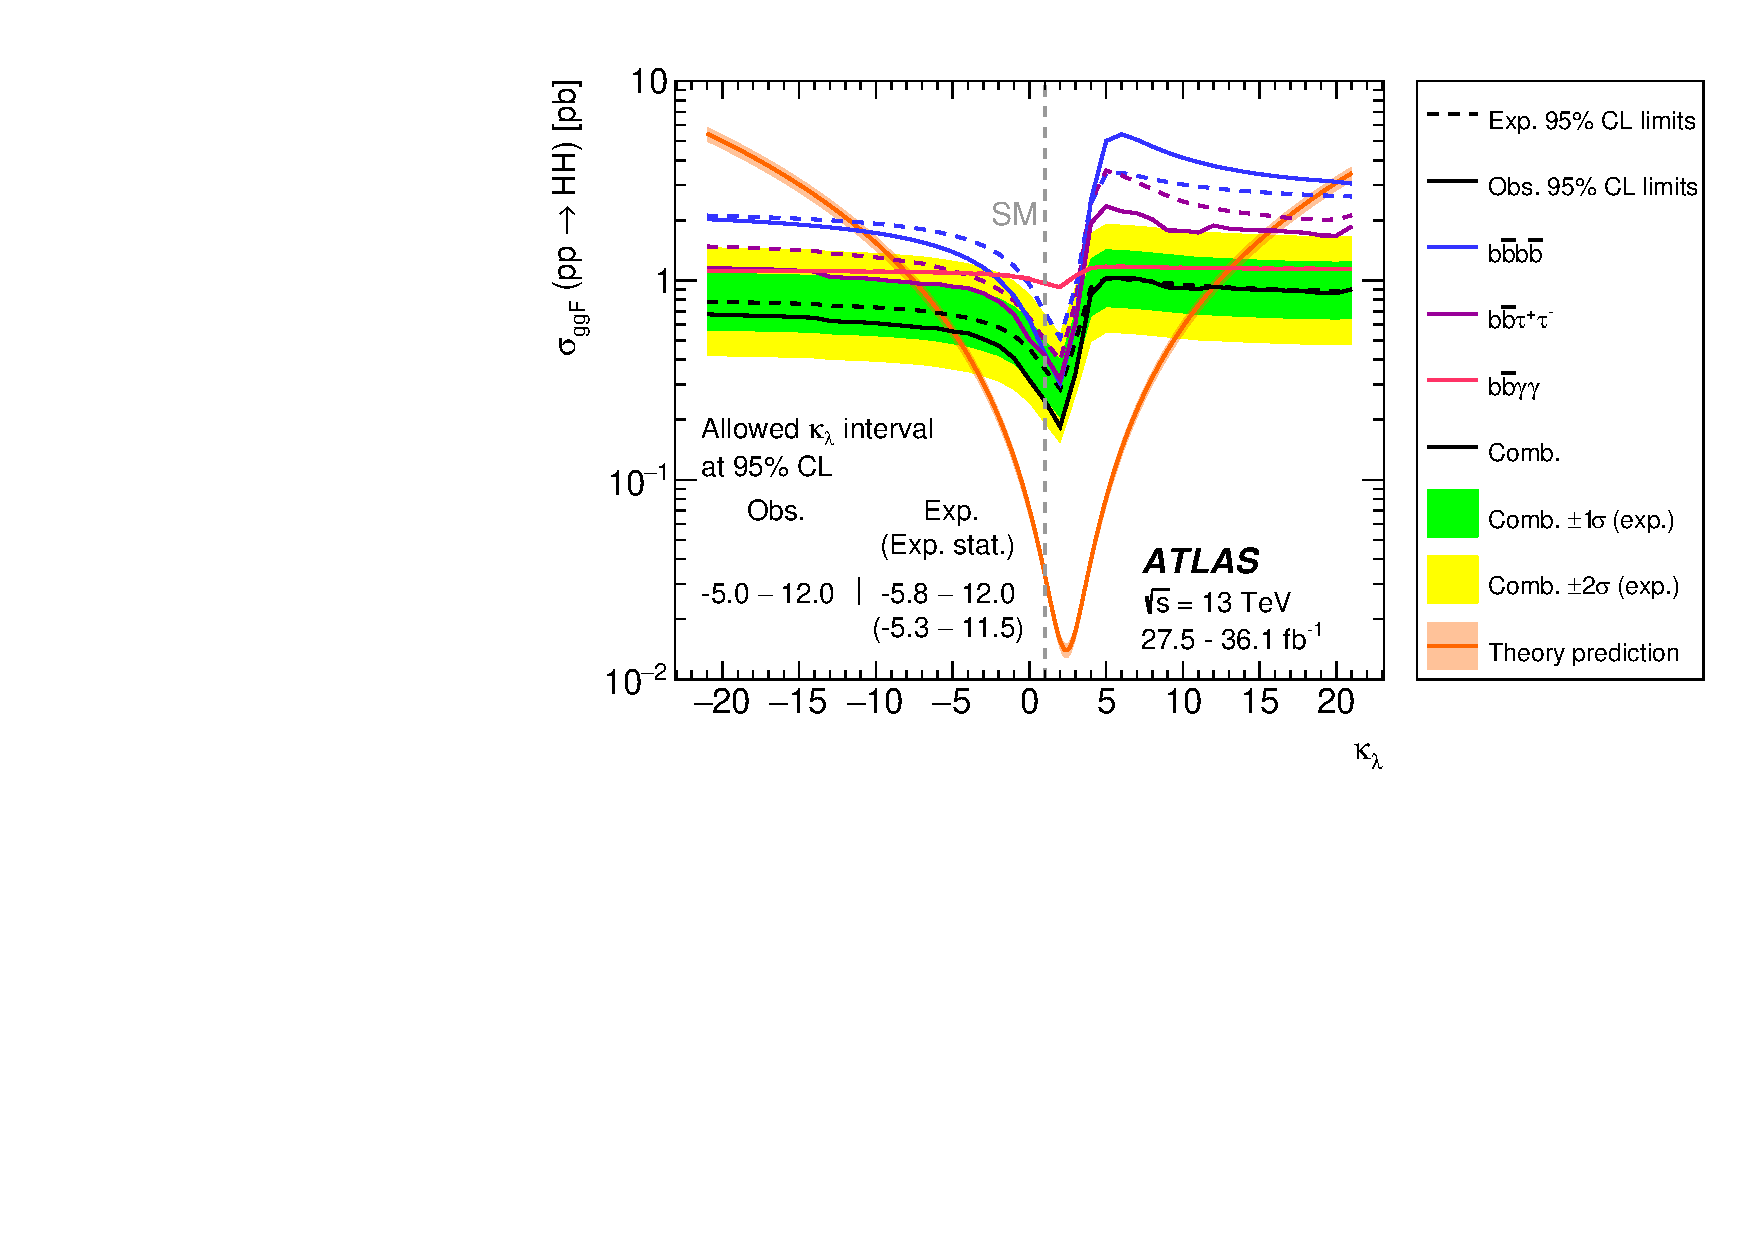
\includegraphics[width=0.67\textwidth, trim=0 1.2em 0 0,
    clip]{status/atlas_36ifb_klambda}

    % trim={<left> <lower> <right> <upper>}

    \subcaption{Results of the ATLAS collaboration for the \bbbb, \bbtautau, and
      \bbyy channels and their combination. The figure is taken from
      Ref.~\cite{HDBS-2018-58}.}
  \end{subfigure}

  \vspace{0.5em}

  \begin{subfigure}[b]{0.9\textwidth}
    \centering

    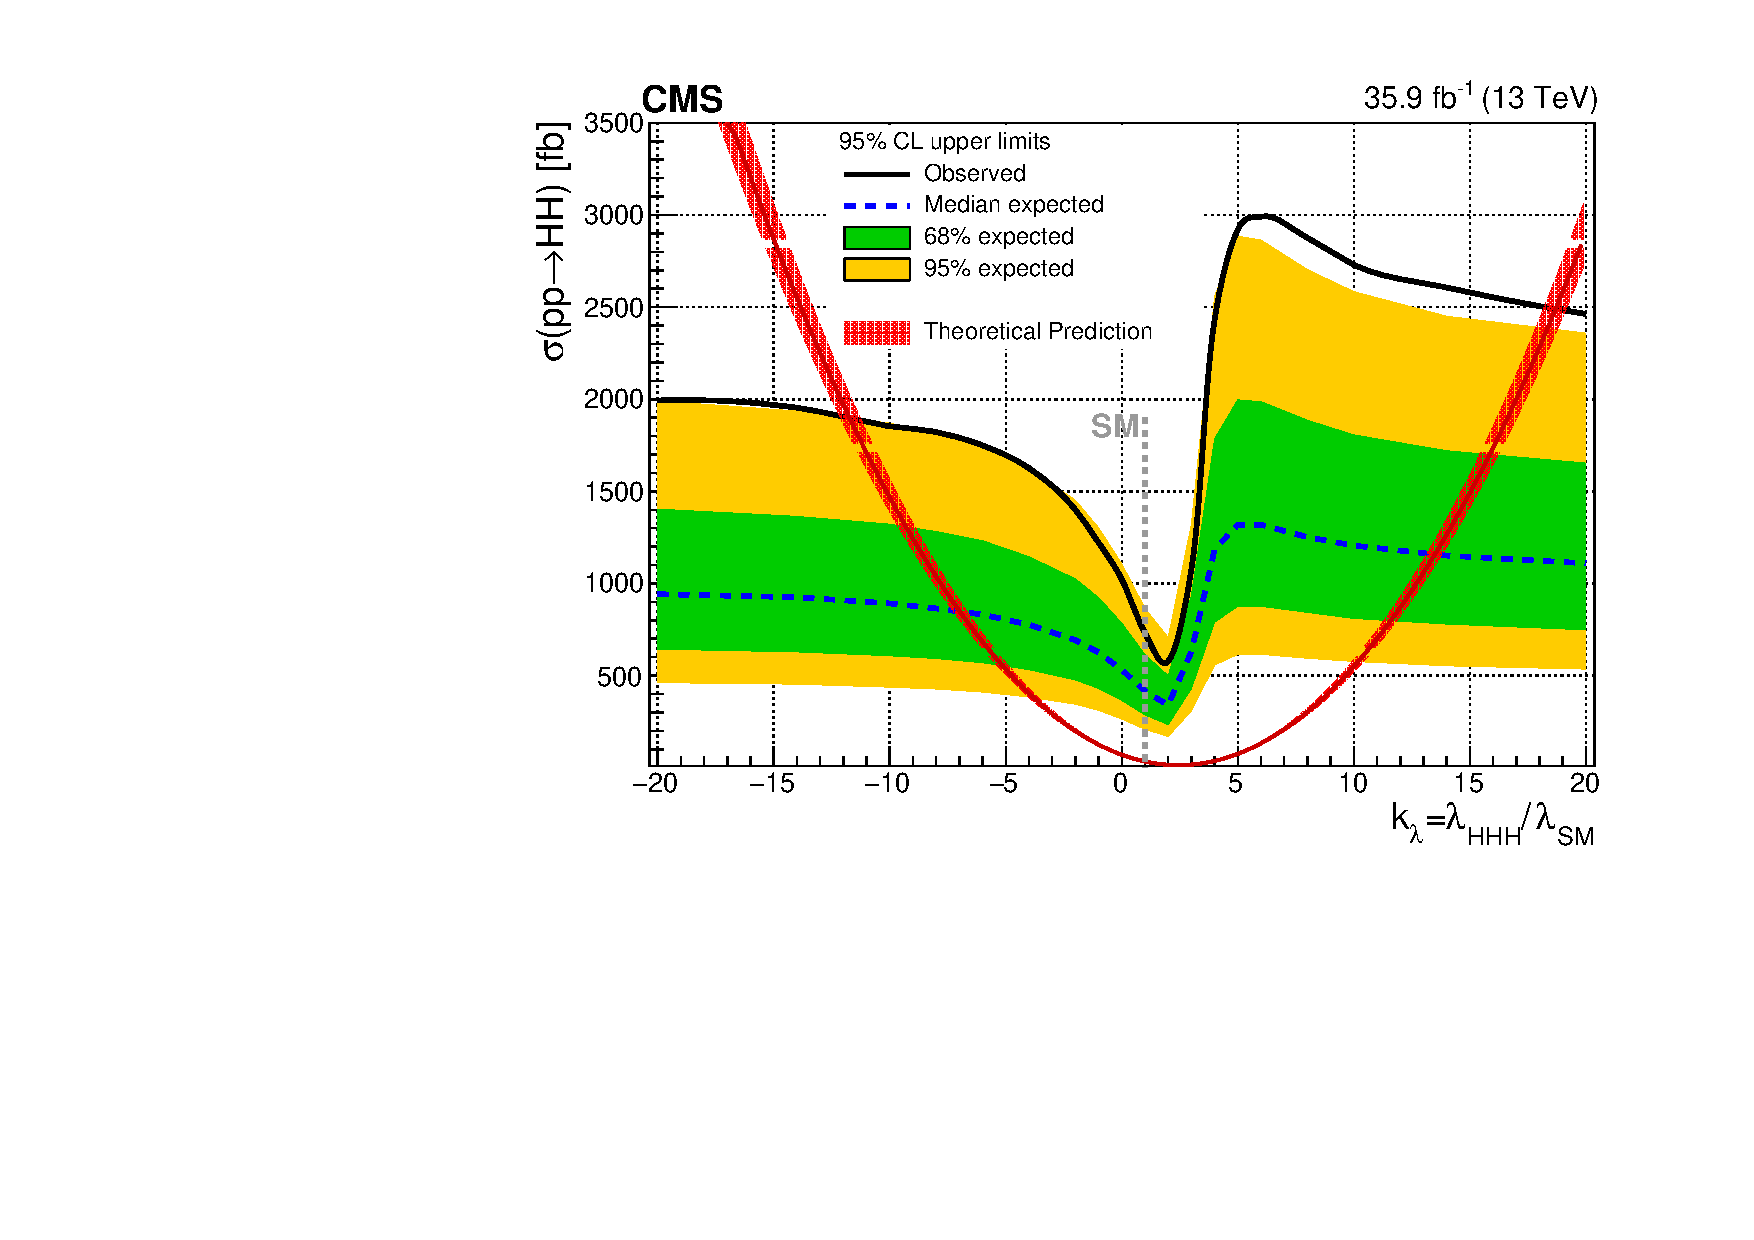
\includegraphics[width=0.58\textwidth]{status/cms_36ifb_klambda}

    \subcaption{Results of the CMS collaboration for the combination of the
      \bbbb, \bbtautau, \bbyy, and $\bbbar VV$ channels. The figure is taken
      from Ref.~\cite{CMS-HIG-17-030}.}
  \end{subfigure}

  \caption[Upper limits on the non-resonant \HH production cross section as a
  function of \klambda by the ATLAS and CMS collaborations based on
  \pp~collision data taken in 2015 and 2016.]{Upper limits at \SI{95}{\percent}
    CL on the cross section of non-resonant \HH production as a function of
    \klambda by the ATLAS (a) and CMS (b) collaborations. The expected upper
    limits are obtained under the background-only assumption (i.e.\ no
    non-resonant \HH production). Values of \klambda where the theoretical
    prediction exceeds the upper limit are excluded by the measurements. The
    results are based on \pp~collision data taken in 2015 and 2016.}%
  \label{fig:prior_status_klambda}
\end{figure}


\subsection*{Searches for Resonant Production of Higgs Boson Pairs}%
\label{sec:past_results_resonant}

The ATLAS and CMS collaborations performed searches for CP-even, scalar
resonances with narrow width decaying into a pair of SM Higgs bosons. Resonance
masses ranging from the \HH production threshold up to \SI{3000}{\GeV} are
considered by both collaborations. The upper limits at \SI{95}{\percent} CL on
the production cross section of the scalar resonance as a function of its mass
are shown in \Cref{fig:prior_status_reso}. Neither the ATLAS nor the CMS result
shows a statistically significant excess in the search for resonant \HH
production.
% The excluded cross sections range from about \SI{1000}{\femto\barn} at low
% mass to about \SI{5}{\femto\barn} at high resonance mass.

\begin{figure}[htbp]
  \centering

  \newcommand*{\mybox}[1][red]{\textcolor{#1}{\rule{1.2ex}{1.2ex}}}
  \definecolor{cbbww}{RGB}{0, 153, 0}
  \definecolor{cbbtautau}{RGB}{153, 0, 153}
  \definecolor{cbbyy}{RGB}{255, 51, 102}
  \definecolor{cbbbb}{RGB}{51, 51, 255}
  \definecolor{cwwyy}{RGB}{0, 204, 204}
  \definecolor{cwwww}{RGB}{204, 102, 51}

  \begin{subfigure}[t]{0.90\textwidth}
    \centering

    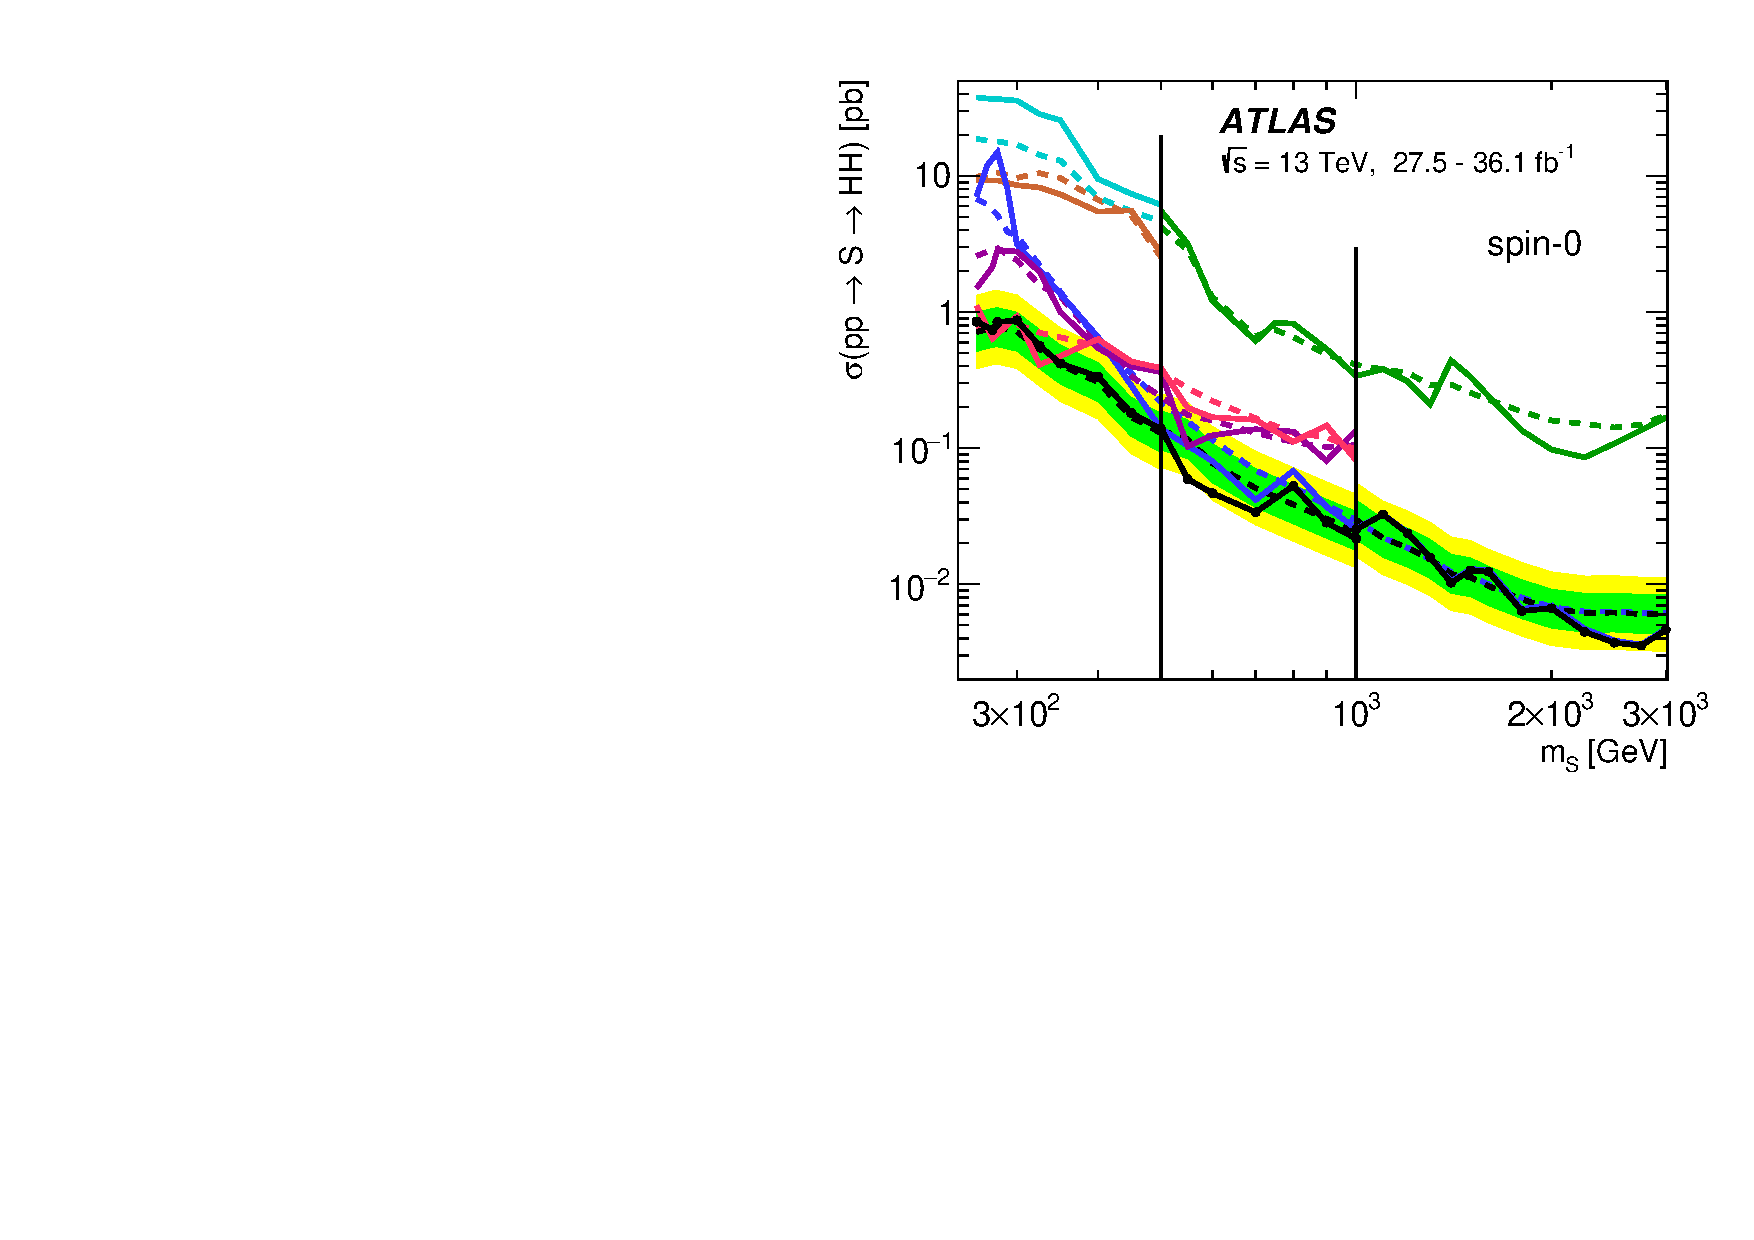
\includegraphics[width=0.52\textwidth, trim=0 0.2em 0 0,
    clip]{status/atlas_36ifb_resonant}

    \subcaption{Results of the ATLAS collaboration for the channels:
      \bbbb~(\mybox[cbbbb]), \bbtautau~(\mybox[cbbtautau]),
      \bbyy~(\mybox[cbbyy]), $\bbbar W^+ W^-$~(\mybox[cbbww]),
      $W^+ W^- \gamma\gamma$~(\mybox[cwwyy]), and
      $W^+ W^- W^+ W^-$~(\mybox[cwwww]). The statistical combination of all
      channels is shown in black. The observed (expected) upper limits are
      depicted as solid (dashed) lines. The figure is taken from
      Ref.~\cite{HDBS-2018-58}.}
  \end{subfigure}

  \vspace{0.5em}

  \begin{subfigure}[t]{0.9\textwidth}
    \centering

    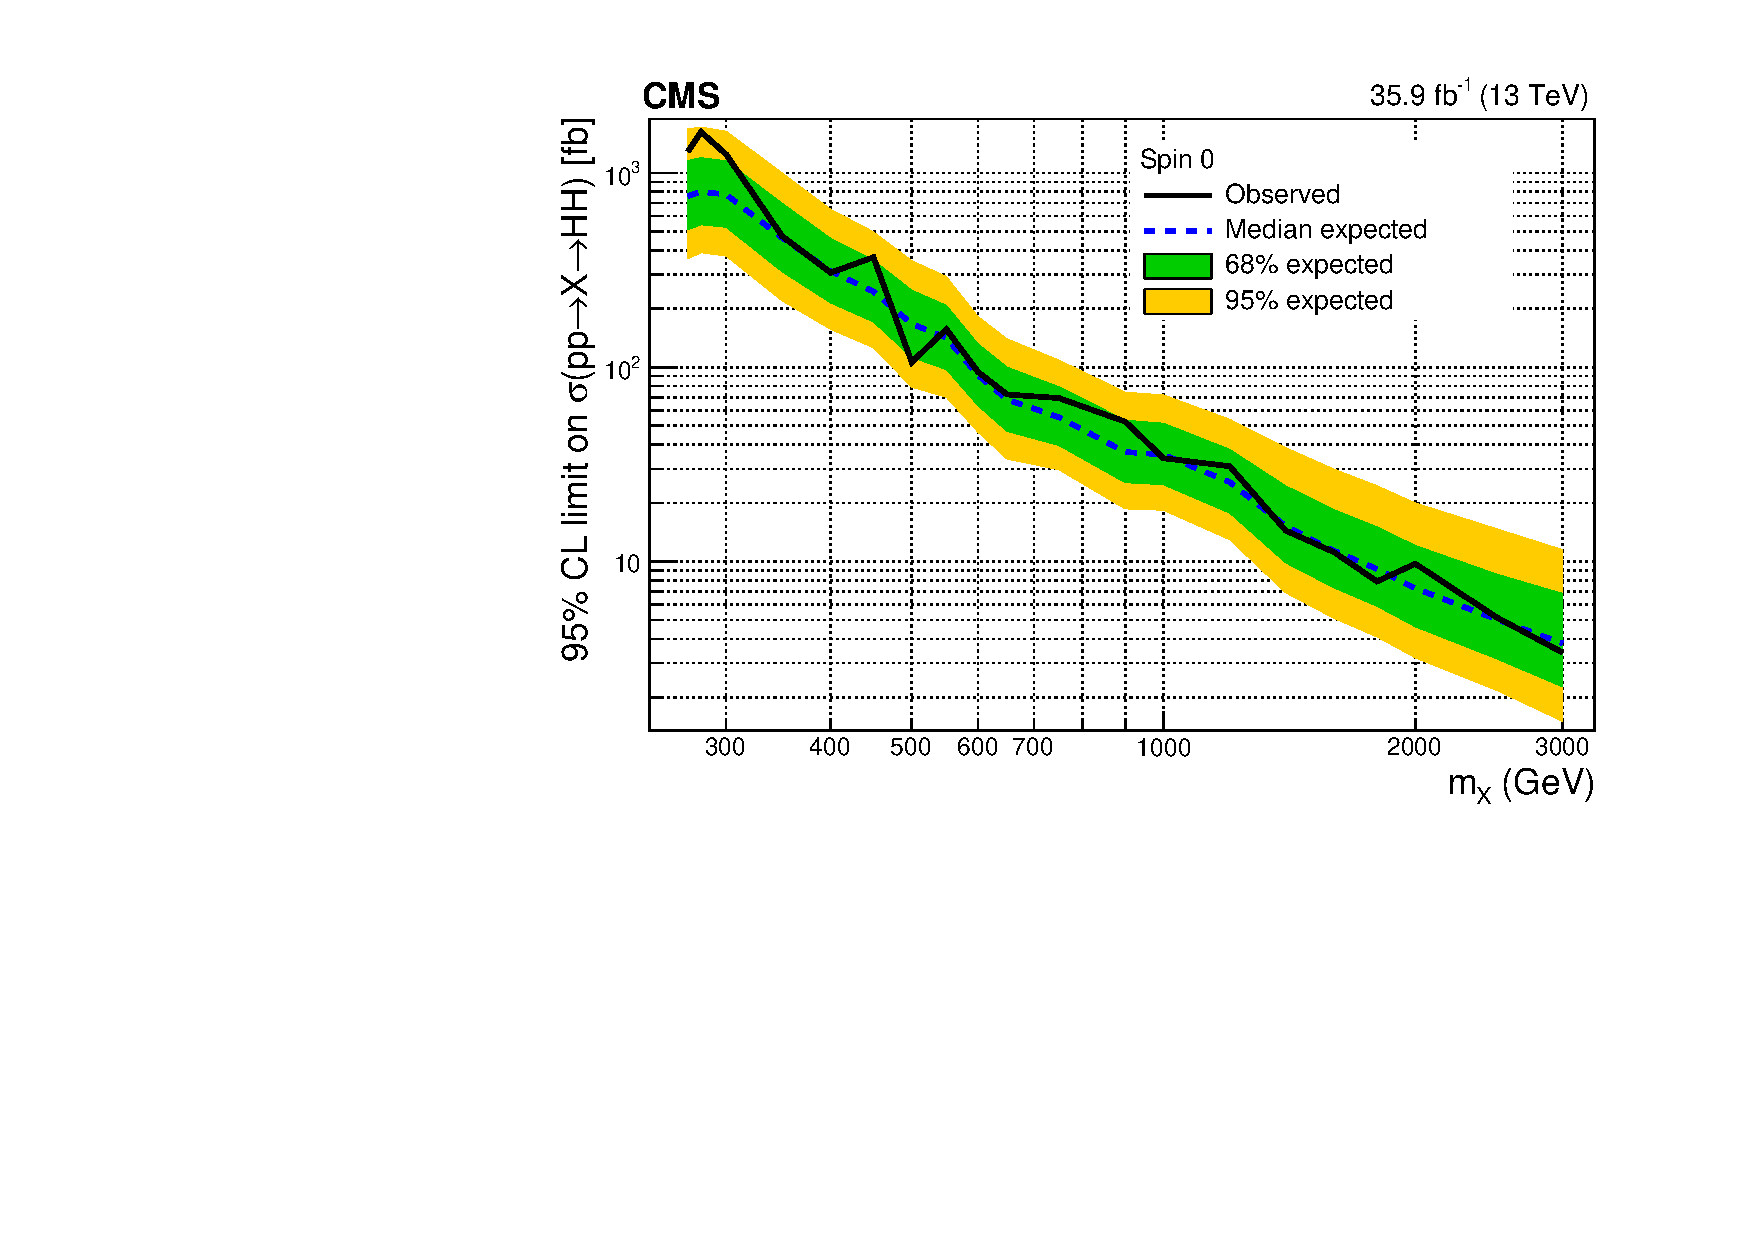
\includegraphics[width=0.6\textwidth]{status/cms_36ifb_resonant}

    \subcaption{Results of the CMS collaboration for the statistical combination
      of the \bbbb, \bbtautau, \bbyy, and $\bbbar VV$ ($V = Z$ or $W^\pm$)
      channels. The figure is taken from Ref.~\cite{CMS-HIG-17-030}.}
  \end{subfigure}

  \caption[Upper limits on the resonant \HH production cross section via scalar,
  narrow-width resonances by the ATLAS and CMS collaborations based on
  \pp~collision data taken in 2015 and 2016.]{Upper limits at \SI{95}{\percent}
    CL on the production cross section of CP-even, scalar resonances ($S$ / $X$)
    decaying into a pair of SM Higgs bosons by the ATLAS (a) and CMS (b)
    collaboration. The expected upper limits are derived assuming the
    background-only hypothesis. The results are based on \pp~collision data
    taken in 2015 and 2016.}%
  \label{fig:prior_status_reso}
\end{figure}


%%% Local Variables:
%%% mode: latex
%%% TeX-master: "../../phd_thesis"
%%% End:
